\documentclass[12pt, times new roman, a4paper]{report}
\usepackage[utf8]{inputenc}
\usepackage{graphicx}

\title{Tugas Besar}
\author{aditya luthfi maulana harahap }
\date{Desember 2019}

\begin{document}

\maketitle
\chapter{Membuat Aplikasi Menggunakan Oracle Apex}

\section{Oracle Application Express (APEX)}

\hspace{1cm} Oracle Application Express (Oracle APEX) yang dulu disebut HTML-DB adalah sebuah framework yang berbasis pada sebuah database dedicated (sementara ini sampai versi terbaru masih dedicated untuk Oracle Db saja dan lisensi include dalam lisensi database), ini artinya apa bahwa engine aplikasi dibangun sepenuhnya didalam sebuah database. Bahkan untuk arsitektur Embedded PL/SQL Gateway seperti yang dipakai dalam Oracle XE dan Oracle 11G file image (library,css,theme,dll) disimpan didalam database metadata juga. Inilah hal yang berbeda dibandingkan framework yang lain.

\subsection{Cara Mengakses APEX}
\hspace{1cm} Oracle APEX dapat di akses secara online ataupun offline.

\begin{enumerate}
\item Offline\\
	\hspace{1cm} Dapat di download disini 	: https://www.oracle.com/tools/	   downloads/apex-downloads.html
\item Online\\
	\hspace{1cm} Dapat di akses disini : https://apex.oracle.com/en/
\end{enumerate}

\par Disini saya menggunakan APEX online. untuk mengakses nya silahkan klik link yang telah disediakan diatas. Setelah masuk ke situsnya anda haruslah memiliki akun APEX online terlebih dahulu untuk mengaksesnya.\\
\par Jika anda belum memiliki akun silahkan daftar dengan mengklik \textit{Get Started for Free}, lalu isi data-data yang diminta. Jika telah memiliki akun silahkan login dengan klik \textit{sign in} dan masukkan \textit{Workspace, Username, Password} anda.

\section{Merancang database di APEX Online}
\subsection{Membuat Database di APEX}
\hspace{1cm} Untuk membuat database bisa upload tabel melalui excel dan juga dibuat langsung melalui \textit{SQL Commads}, tetapi disini saya ditugaskan untuk membuat tabel melalui \textit{SQL Commads}.\\
\\
Berikut langkah-langkah untuk menjalankan \textit{SQL Commands} :

\begin{enumerate}

\item Klik SQL Workshop
\begin{figure} [h]
	\centering
		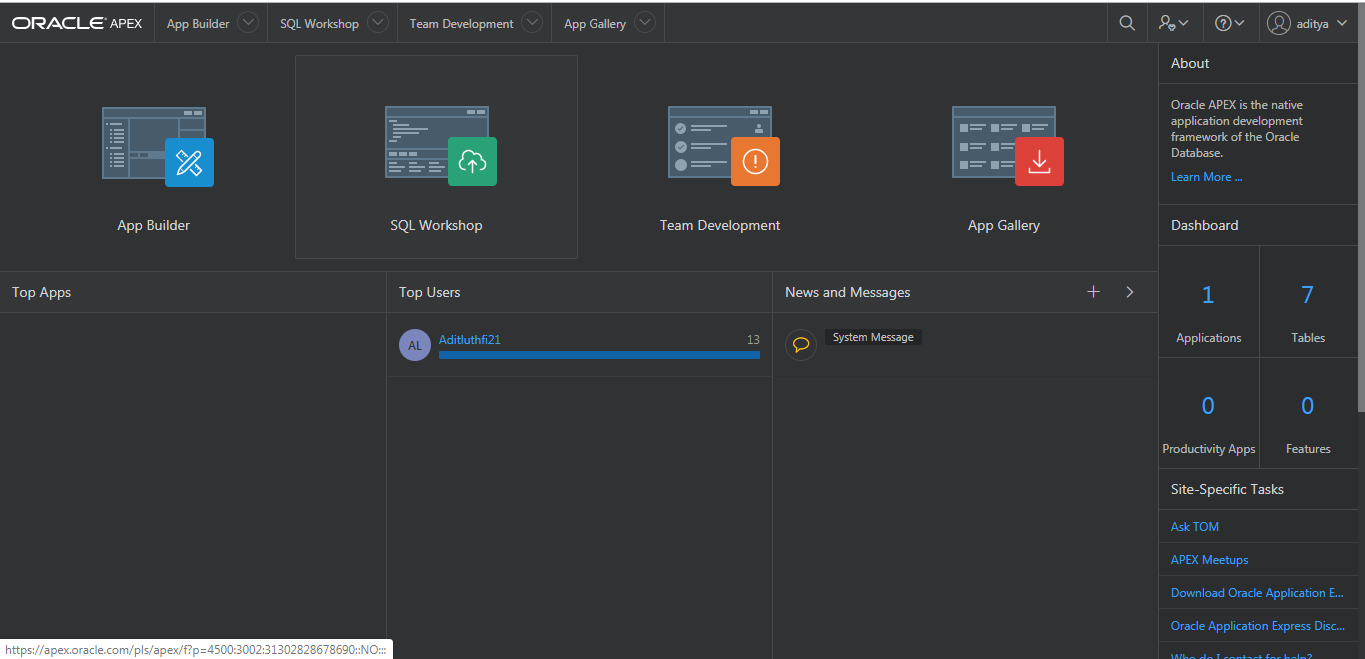
\includegraphics[scale=0.25]{gambar/1}
\end{figure}

\item Lalu Klik SQL Commands
\begin{figure} [h]
	\centering
		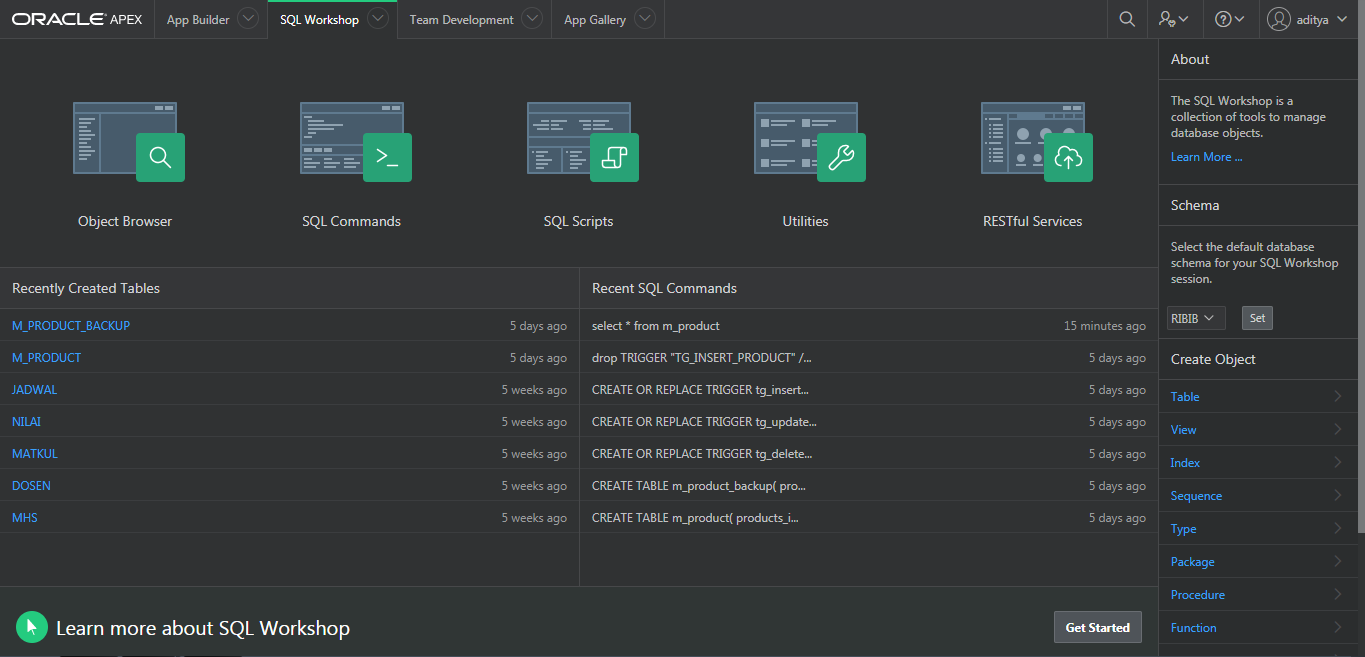
\includegraphics[scale=0.25]{gambar/2}
\end{figure}
\\
\\	
\item Beginilah tampilan SQL Commands, dan disinilah anda memasukkan perintah-perintah SQL.
\begin{figure} [h]
	\centering
		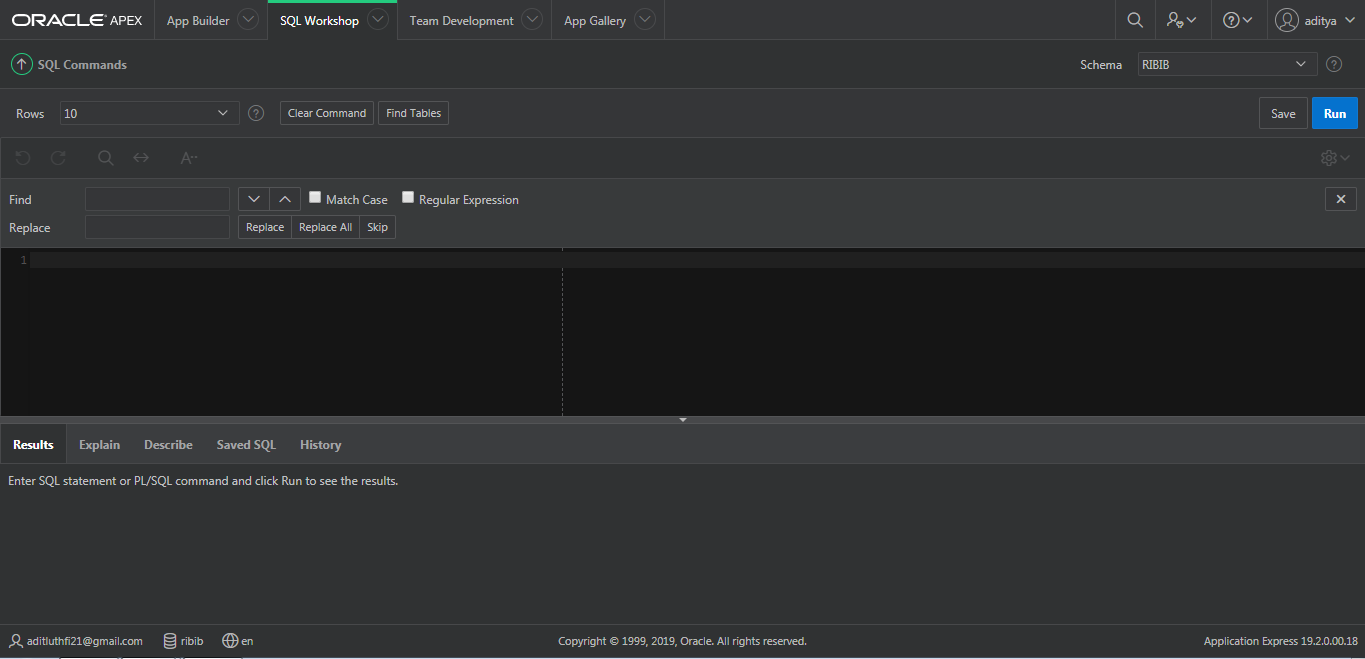
\includegraphics[scale=0.3]{gambar/3}
\end{figure}
\end{enumerate}

\subsection{Membuat tabel database}
\subsubsection{Membuat table pegawai}
\hspace{1cm} Table ini berfungsi untuk menampung data pegawai\\
\\
Ketikkan query berikut di SQL Command :\\
\\
CREATE TABLE pegawai(\\
 pegawai\textunderscore id number(5) not null primary key,\\
 nama\textunderscore pegawai varchar(55),\\
 gaji number(15),\\
 jabatan\textunderscore id number(5) not null\\
)\\
\begin{figure}[h]
	\centering
		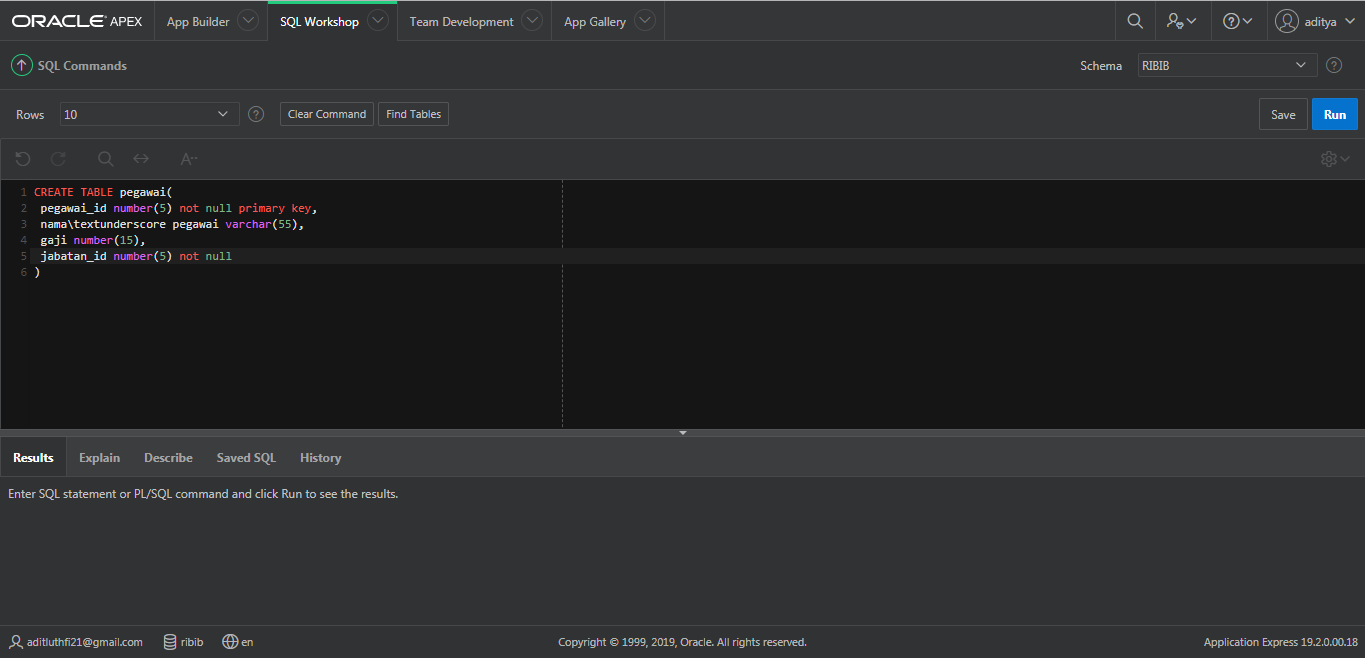
\includegraphics[scale=0.3]{gambar/5}
\end{figure}
\\
\\
\par hasilnya akan seperti ini :
\begin{figure}[h]
	\centering
		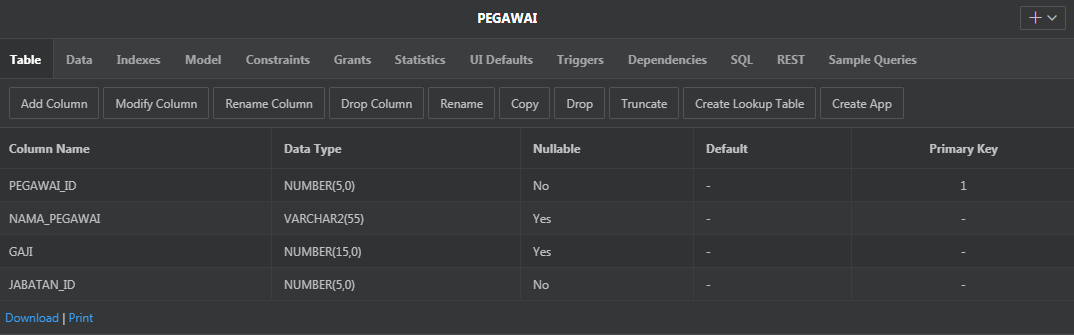
\includegraphics[scale=0.5]{gambar/4}
\end{figure}

\subsubsection{Membuat table pegawai\textunderscore backup}
\hspace{1cm} Table ini berfungsi sebagai backup dari table pegawai apabila record dari table pegawai di manipulasi(insert,update,delete)\\
\\
Ketikkan query berikut di SQL Command :\\
\\
CREATE TABLE pegawai\textunderscore backup(\\
 pegawai\textunderscore id number(5) not null,\\
 nama\textunderscore pegawai varchar(55),\\
 gaji number(15),\\
 jabatan\textunderscore id number(5)\\
 change\textunderscore at timestamp,\\
 changed\textunderscore type varchar(255)
)\\
\begin{figure}[h]
	\centering
		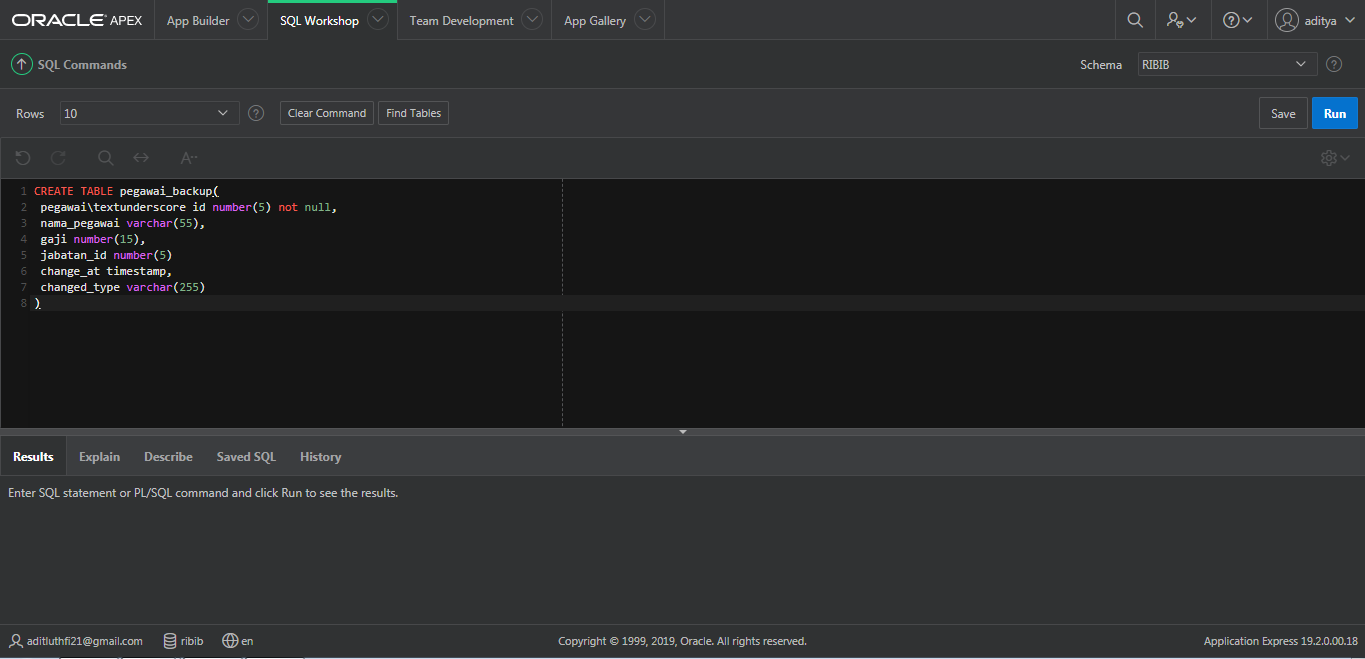
\includegraphics[scale=0.3]{gambar/6}
\end{figure}
\\
\\
\par hasilnya akan seperti ini :
\begin{figure}[h]
	\centering
		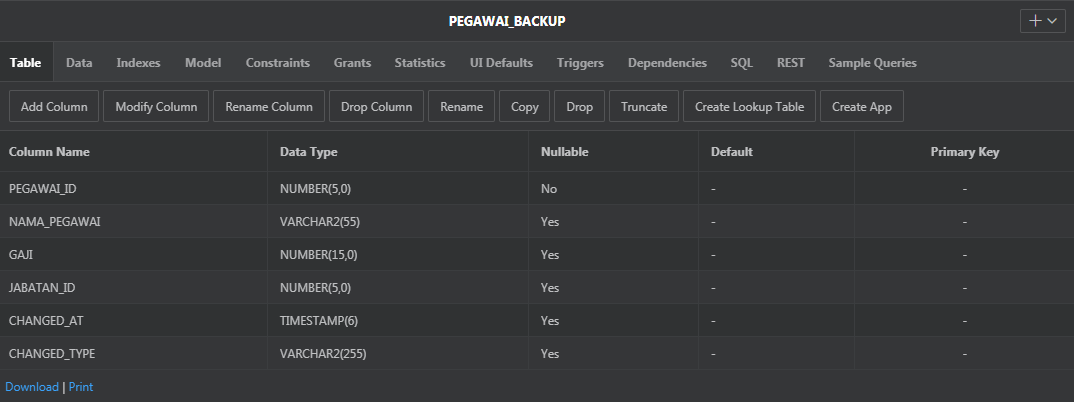
\includegraphics[scale=0.5]{gambar/7}
\end{figure}

\subsubsection{Membuat Table jabatan}
\hspace{1cm} Table ini berfungsi untuk menampung data jabatan.\\
\\
Ketikkan query berikut di SQL Command :\\
\\
CREATE TABLE jabatan(\\
 jabatan\textunderscore id number(5) not null primary key,\\
 nama\textunderscore jabatan varchar(55),\\
)
\begin{figure}[h]
	\centering
		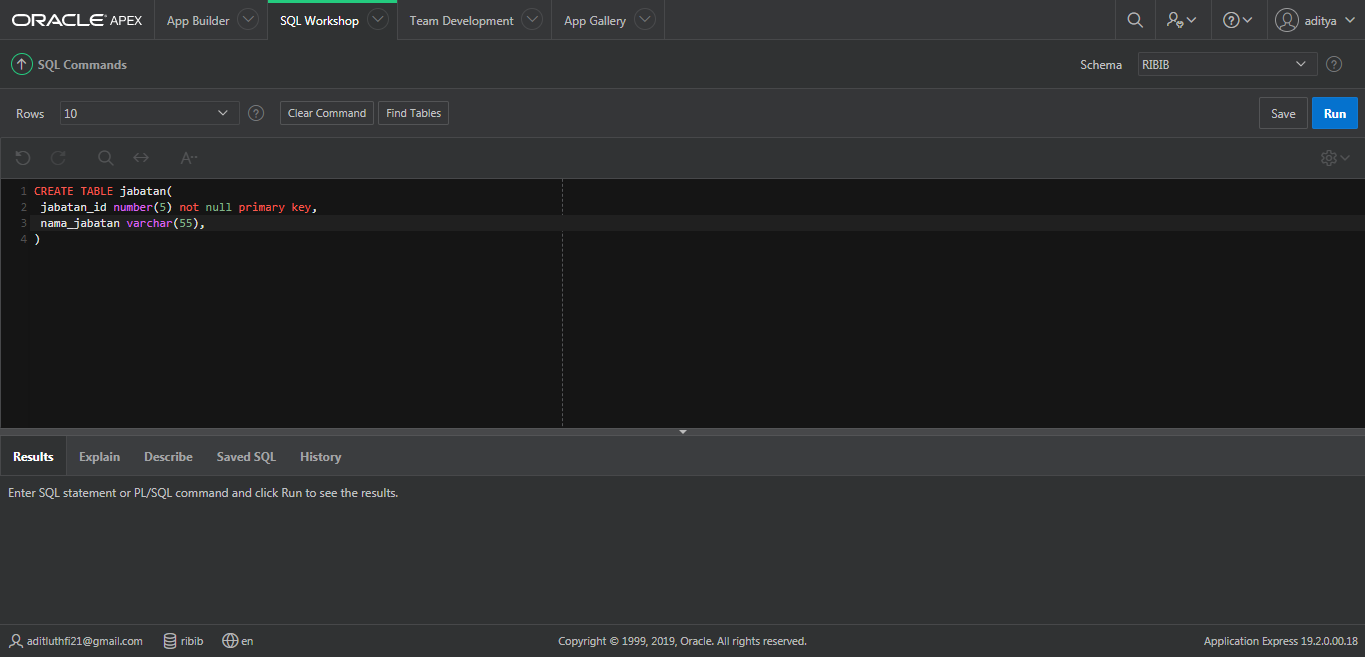
\includegraphics[scale=0.4]{gambar/8}
\end{figure}

\par hasilnya akan seperti ini :
\begin{figure}[h]
	\centering
		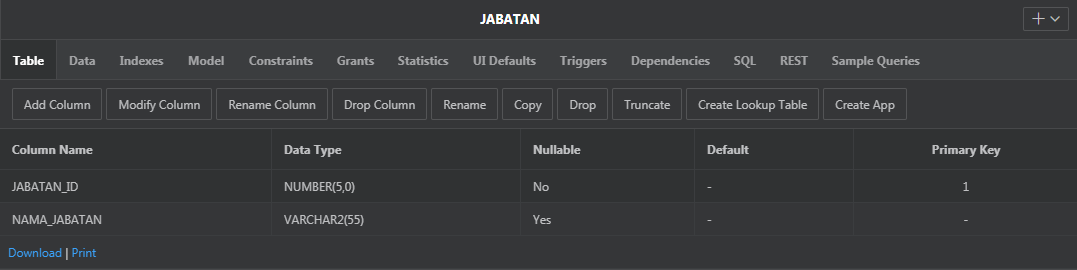
\includegraphics[scale=0.5]{gambar/9}
\end{figure}

\subsubsection{Membuat table jabatan\textunderscore backup}
\hspace{1cm} Table ini berfungsi sebagai backup dari table jabatan apabila record dari table jabatan di manipulasi(insert,update,delete)\\
\\
Ketikkan query berikut di SQL Command :\\
\\
CREATE TABLE  JABATAN\textunderscore BACKUP\\ 
   (	JABATAN\textunderscore ID NUMBER(5,0) NOT NULL ENABLE,\\ 
	NAMA\textunderscore JABATAN VARCHAR2(55),\\
	CHANGED\textunderscore AT TIMESTAMP,\\ 
	CHANGED\textunderscore TYPE VARCHAR2(25)\\
   )
\begin{figure}[h]
	\centering
		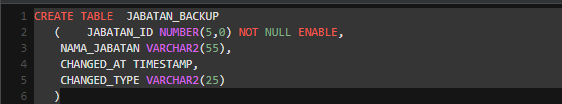
\includegraphics[scale=0.8]{gambar/15}
\end{figure}   
\par hasilnya akan seperti ini :
\begin{figure}[h]
	\centering
		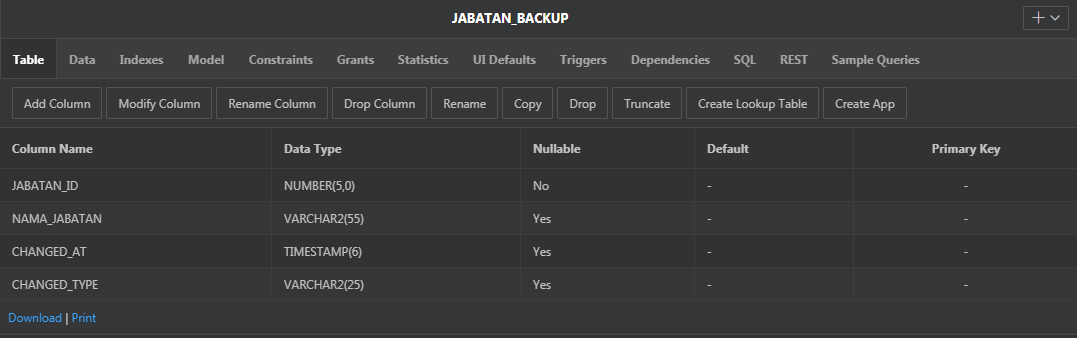
\includegraphics[scale=0.4]{gambar/16}
\end{figure}

\subsection{Membuat relasi antar table}
\hspace{1cm} Relasi digunakan sebagai penghubung antar table yang saling berhubungan. Untuk Menghubungkan table menggunakan foreign key, foreign key di dapatkan dari primary key table.
\\
\par Ketikkan query berikut di SQL Commands :\\
\\
ALTER TABLE  PEGAWAI ADD FOREIGN KEY (JABATAN\textunderscore ID)\\
	  REFERENCES  JABATAN (JABATAN\textunderscore ID)
\begin{figure}[h]
	\centering
		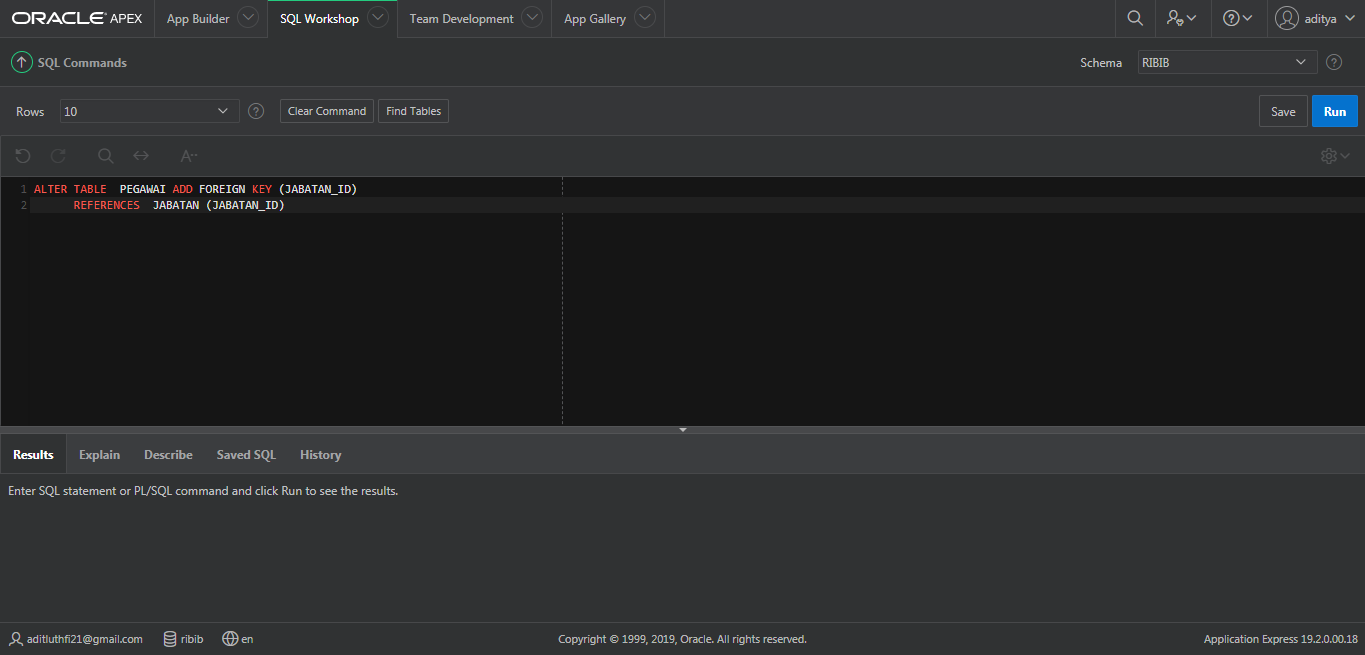
\includegraphics[scale=0.3]{gambar/10}
\end{figure}
\par Hasilnya akan seperti ini :
\begin{figure}[h]
	\centering
		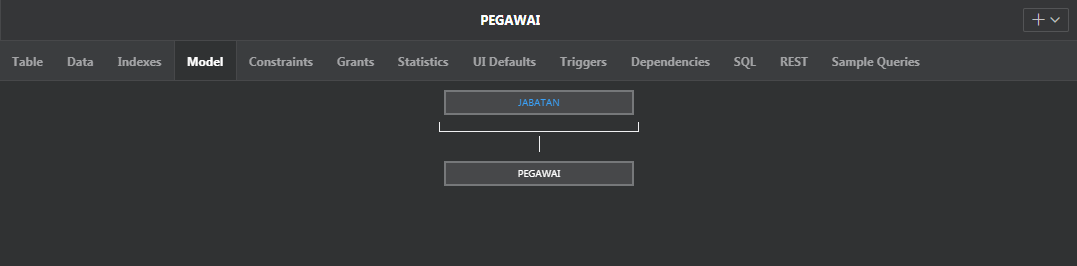
\includegraphics[scale=0.5]{gambar/11}
\end{figure}
\\
\\
\\
\\
\\
\\
\\
\\
\subsection{Trigger}
\hspace{1cm} Trigger Database adalah sesuatu perintah yang kita siapan untuk berjalan otomatis ketika perintah tertentu(insert, update, delete) dijalankan.

\subsubsection{Membuat Trigger insert}
\begin{enumerate}
\item Trigger insert pegawai\\
Trigger insert berfungsi jika ada memasukkan record baru ke dalam table pegawai maka recordnya juga masuk ke dalam table pegawai\textunderscore backup\\
\par Ketikkan query berikut pada SQL Commands :\\
\\
create or replace TRIGGER insert\textunderscore pegawai\\
AFTER insert ON pegawai\\
FOR EACH ROW\\
BEGIN\\
    insert into pegawai\textunderscore backup values (\\
        :new.pegawai\textunderscore id,\\
        :new.nama\textunderscore pegawai,\\
        :new.gaji,\\
        :new.jabatan\textunderscore id,\\
        CURRENT\textunderscore TIMESTAMP,\\
        'insert'\\
        );\\
END;
\begin{figure}[h]
	\centering
		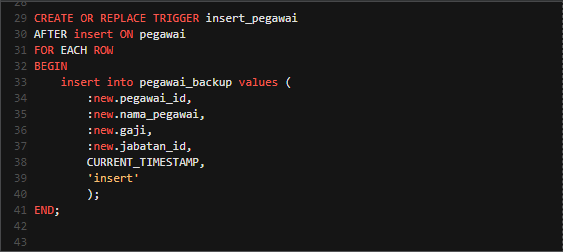
\includegraphics[scale=0.7]{gambar/12}
\end{figure}

\item Trigger insert jabatan\\
Trigger insert berfungsi jika ada memasukkan record baru ke dalam table jabatan maka recordnya juga masuk ke dalam table jabatan\textunderscore backup\\
\par Ketikkan query berikut pada SQL Commands :\\
\\
create or replace TRIGGER insert\textunderscore jabatan\\
AFTER insert ON jabatan\\
FOR EACH ROW\\
BEGIN\\
    insert into jabatan\textunderscore backup values (\\
        :new.jabatan\textunderscore id,\\
        :new.nama\textunderscore jabatan,\\
        CURRENT\textunderscore TIMESTAMP,\\
        'insert'\\
        );\\
END;
\begin{figure}[h]
	\centering
		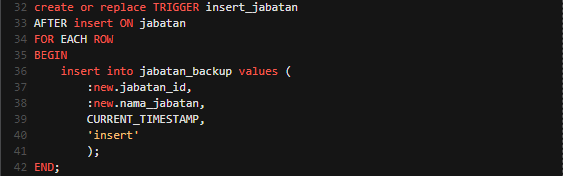
\includegraphics[scale=0.7]{gambar/17}
\end{figure}

\end{enumerate}


\subsubsection{Membuat Trigger update}
\begin{enumerate}
\item Trigger update pegawai\\
Trigger update berfungsi jika record pada table pegawai diubah maka data sebelum di ubah akan masuk ke table pegawai\textunderscore backup\\
\par Ketikkan query berikut pada SQL Commands :\\
\\
create or replace TRIGGER update\textunderscore pegawai\\
AFTER update ON pegawai\\
FOR EACH ROW\\
BEGIN\\
    insert into pegawai\textunderscore backup values (\\
        :old.pegawai\textunderscore id,\\
        :old.nama\textunderscore pegawai,\\
        :old.gaji,\\
        :old.jabatan\textunderscore id,\\
        CURRENT\textunderscore TIMESTAMP,\\
        'update'\\
        );\\
END;
\begin{figure}[h]
	\centering
		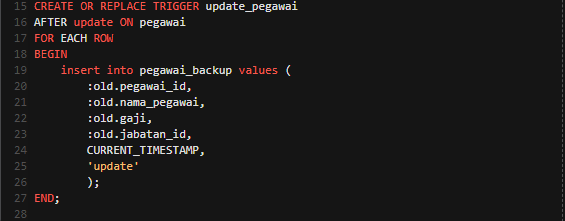
\includegraphics[scale=0.7]{gambar/13}
\end{figure}

\item Trigger update jabatan\\
Trigger update berfungsi jika record pada table jabatan diubah maka data sebelum di ubah akan masuk ke table jabatan\textunderscore backup\\
\par Ketikkan query berikut pada SQL Commands :\\
\\
create or replace TRIGGER update\textunderscore jabatan\\
AFTER update ON jabatan\\
FOR EACH ROW\\
BEGIN\\
    insert into jabatan\textunderscore backup values (\\
        :old.jabatan\textunderscore id,\\
        :old.nama\textunderscore jabatan,\\
        CURRENT\textunderscore TIMESTAMP,\\
        'update'\\
        );\\
END;
\begin{figure}[h]
	\centering
		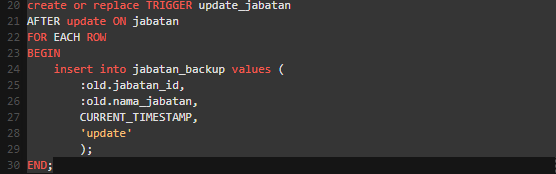
\includegraphics[scale=0.7]{gambar/18}
\end{figure}
\end{enumerate}


\subsubsection{Membuat Trigger delete}
\begin{enumerate}
\item Trigger delete pegawai\\
Trigger delete berfungsi jika record pada table pegawai dihapus maka akan recordnya akan masuk ke table pegawai\textunderscore backup\\
\par Ketikkan query berikut pada SQL Commands :\\
\\
create or replace TRIGGER delete\textunderscore pegawai\\
AFTER DELETE ON pegawai\\
FOR EACH ROW\\
BEGIN\\
    insert into pegawai\textunderscore backup values (\\
        :old.pegawai\textunderscore id,\\
        :old.nama\textunderscore pegawai,\\
        :old.gaji,\\
        :old.jabatan\textunderscore id,\\
        CURRENT\textunderscore TIMESTAMP,\\
        'DELETED'\\
        );\\
END;
\begin{figure}[h]
	\centering
		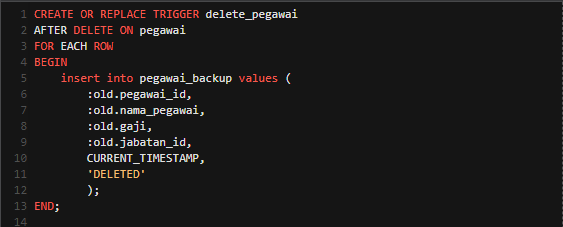
\includegraphics[scale=0.7]{gambar/14}
\end{figure}

\item Trigger delete jabatan\\
Trigger delete berfungsi jika record pada table jabatan dihapus maka akan recordnya akan masuk ke table jabatan\textunderscore backup\\
\par Ketikkan query berikut pada SQL Commands :\\
\\
create or replace TRIGGER delete\textunderscore jabatan\\
AFTER DELETE ON jabatan\\
FOR EACH ROW\\
BEGIN\\
    insert into jabatan\textunderscore backup values (\\
        :old.jabatan\textunderscore id,\\
        :old.nama\textunderscore jabatan,\\
        CURRENT\textunderscore TIMESTAMP,\\
        'DELETED'\\
        );\\
END;
\begin{figure}[h]
	\centering
		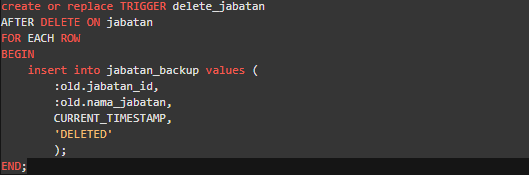
\includegraphics[scale=0.7]{gambar/19}
\end{figure}
\end{enumerate}

\subsection{View}
\hspace{1cm} View adalah perintah query yang disimpan pada database dengan suatu nama tertentu, sehingga bisa digunakan setiap saat untuk melihat data tanpa menuliskan ulang query tersebut.

\subsubsection{Membuat View pada table pegawai\textunderscore backup}
\begin{enumerate}
\item View Insert
\par Ketikkan query berikut pada SQL Commands :\\
\\
 CREATE VIEW pegawai\textunderscore insert AS SELECT*FROM pegawai\textunderscore backup\\
  WHERE CHANGED\textunderscore TYPE='insert';
\begin{figure}[h]
	\centering
		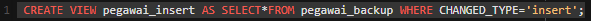
\includegraphics[scale=0.9]{gambar/20}
\end{figure}

\newpage
\item View Update
\par Ketikkan query berikut pada SQL Commands :\\
\\
CREATE VIEW pegawai\textunderscore update AS SELECT*FROM pegawai\textunderscore backup\\ 
\\
WHERE CHANGED\textunderscore TYPE='update';
\begin{figure}[h]
	\centering
		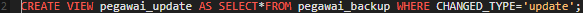
\includegraphics[scale=1]{gambar/21}
\end{figure}

\item View Delete
\par Ketikkan query berikut pada SQL Commands :\\
\\
CREATE VIEW pegawai\textunderscore delete AS SELECT*FROM pegawai\textunderscore backup WHERE CHANGED\textunderscore TYPE='DELETED';
\begin{figure}[h]
	\centering
		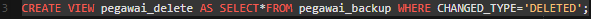
\includegraphics[scale=1]{gambar/22}
\end{figure}
\end{enumerate}

\newpage
\subsubsection{Membuat View pada table jabatan\textunderscore backup}
\begin{enumerate}
\item View Insert
\par Ketikkan query berikut pada SQL Commands :\\
\\
CREATE VIEW jabatan\textunderscore insert AS SELECT*FROM jabatan\textunderscore backup WHERE CHANGED\textunderscore TYPE='insert';
\begin{figure}[h]
	\centering
		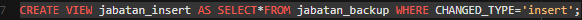
\includegraphics[scale=1]{gambar/23}
\end{figure}

\item View Update
\par Ketikkan query berikut pada SQL Commands :\\
\\
CREATE VIEW jabatan\textunderscore update AS SELECT*FROM jabatan\textunderscore backup WHERE CHANGED\textunderscore TYPE='update';
\begin{figure}[h]
	\centering
		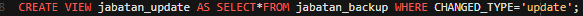
\includegraphics[scale=1]{gambar/24}
\end{figure}

\item View Delete
\par Ketikkan query berikut pada SQL Commands :\\
\\
CREATE VIEW jabatan\textunderscore delete AS SELECT*FROM jabatan\textunderscore backup WHERE CHANGED\textunderscore TYPE='DELETED';
\begin{figure}[h]
	\centering
		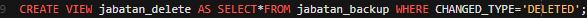
\includegraphics[scale=1]{gambar/25}
\end{figure}
\end{enumerate}

\newpage
\section{Membuat Aplikasi dari rancangan database}
\subsection{ Daftar halaman yang akan dibuat }
\begin{enumerate}
\item Membuat Halaman Form untuk menambahkan data pegawai
\item Membuat Halaman Form untuk menambahkan data jabatan
\item Membuat Halaman Interactive Report Untuk Menampung data penambahan jabatan(View insert table jabatan)
\item Membuat Halaman Interactive Report Untuk Menampung data pegawai masuk(View insert table pegawai)
\item Membuat Halaman Interactive Report Untuk Menampung data pegawai(table pegawai)
\item Membuat Halaman Interactive Report Untuk Menampung data jabatan(table jabatan)
\item Membuat Halaman Interactive Report Untuk Menampung data pegawai backup(table pegawai\textunderscore backup)
\item Membuat Halaman Interactive Report Untuk Menampung data jabatan backup(table jabatan\textunderscore backup)
\end{enumerate}

\subsection{Langkah-langkah membuat aplikasi}
\begin{enumerate}
\item Klik App Builder
\begin{figure}[h]
	\centering
		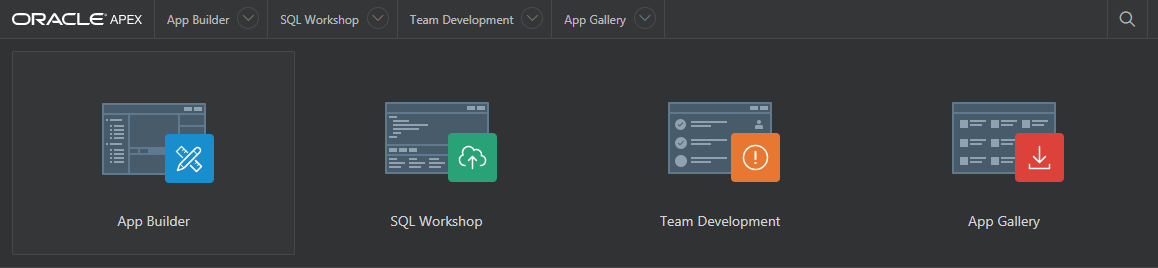
\includegraphics[scale=0.3]{gambar/26}
\end{figure}

\item Lalu klik Create
\begin{figure}[h]
	\centering
		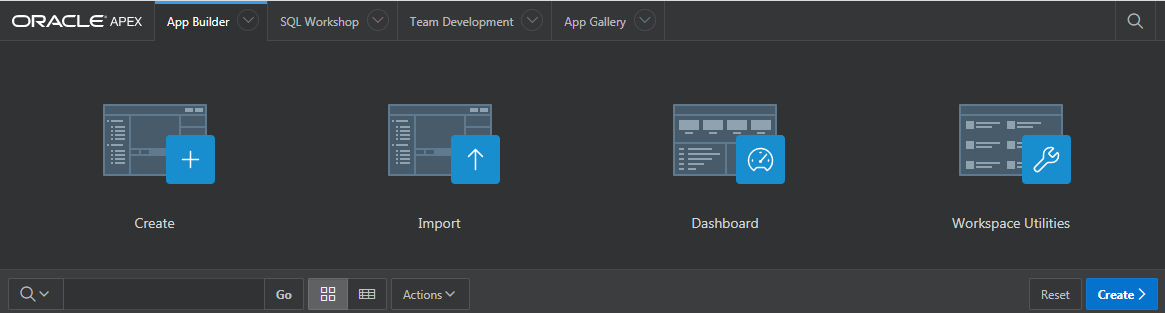
\includegraphics[scale=0.3]{gambar/27}
\end{figure}
\\
\\
\\
\item Kemudian klik New Application
\begin{figure}[h]
	\centering
		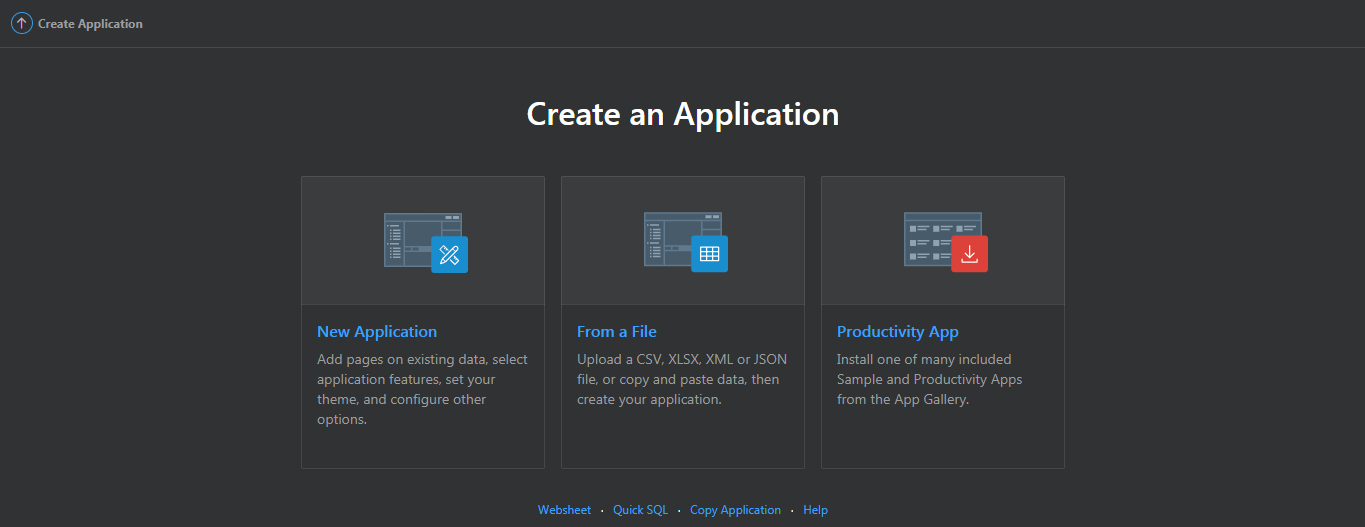
\includegraphics[scale=0.25]{gambar/28}
\end{figure}

\item Setelah itu isi nama aplikasi yang ingin di buat
\begin{figure}[h]
	\centering
		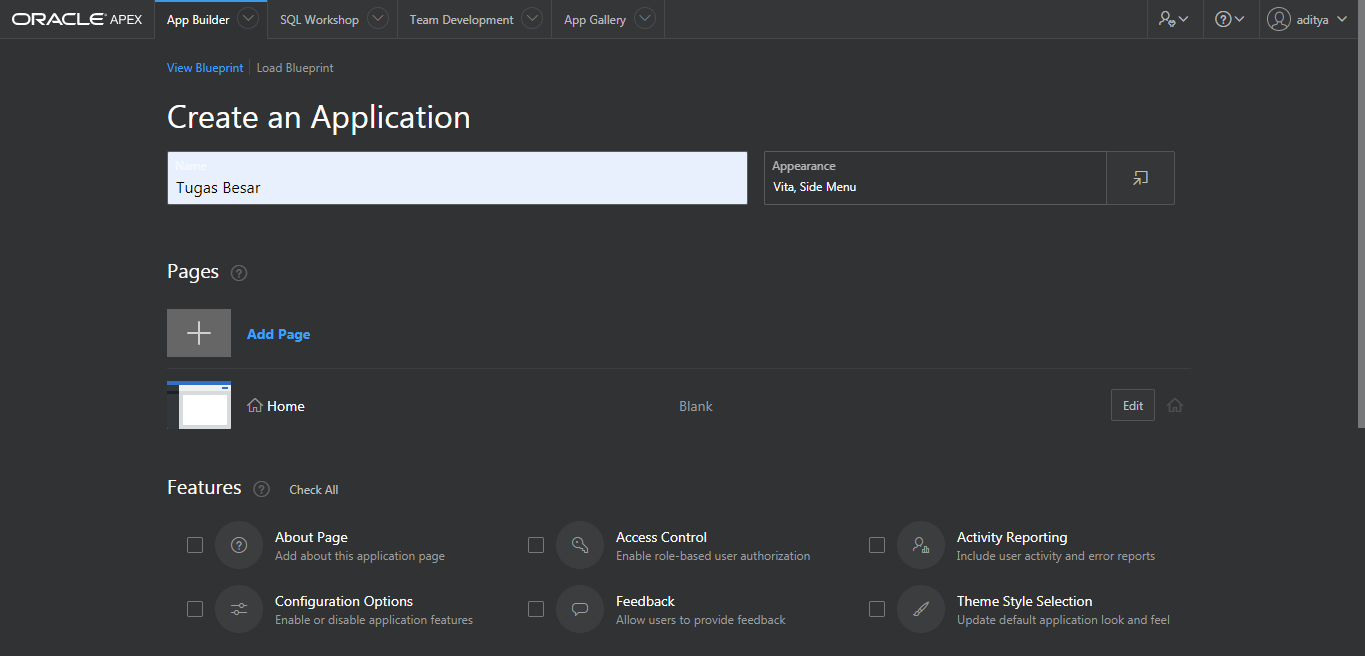
\includegraphics[scale=0.25]{gambar/29}
\end{figure}

\item Selanjutnya klik Add Page untuk membuat halaman. Buatlah Halaman seperti yang sudah di jelaskan di atas.

\item Inilah tampilan Home aplikasi yang sudah dibuat dengan halaman-halaman seperti diatas.
\begin{figure}[h]
	\centering
		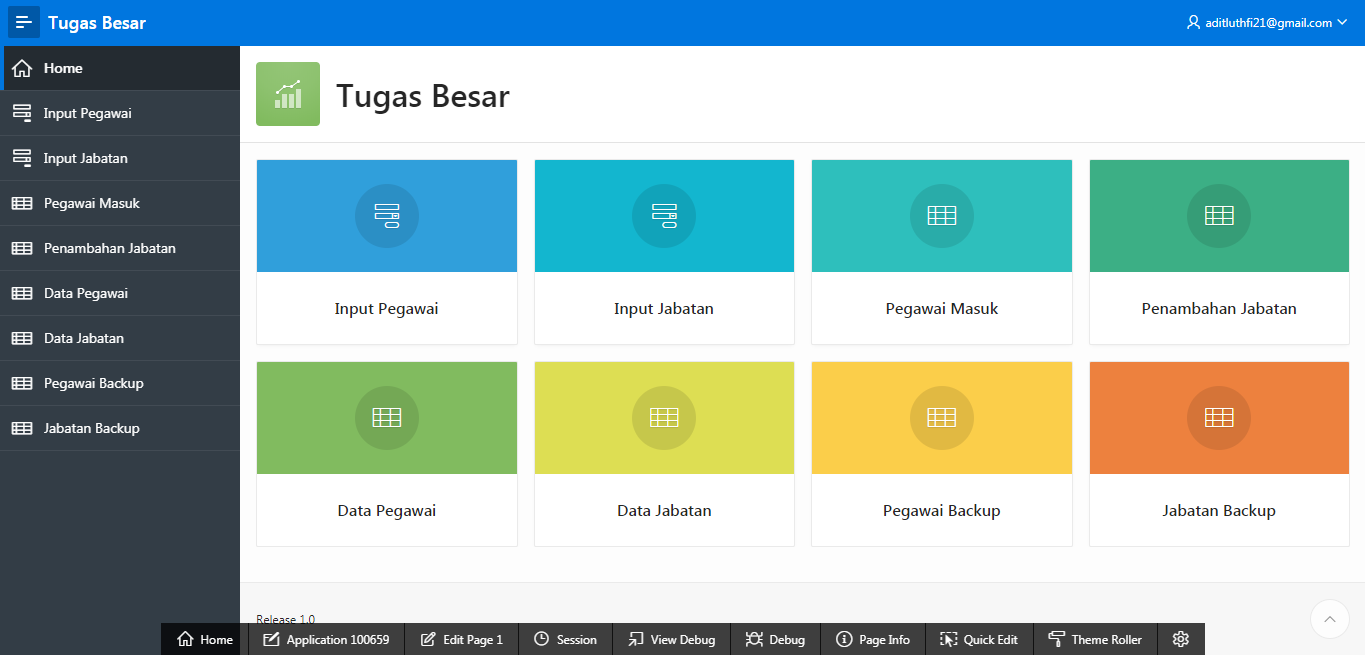
\includegraphics[scale=0.25]{gambar/30}
\end{figure} 
\end{enumerate}

\chapter{Akun}
\section{Login Apex}
\begin{enumerate}
\item Workspace : RIBIB
\item Username : ADITLUTHFI21@GMAIL.COM
\item Password : ribib021
\end{enumerate}

\section{Login Aplikasi}
\begin{enumerate}
\item Link Aplikasi :\\
https://apex.oracle.com/pls/apex/f?p=100659:1:108731702524684:::::
\item Username : aditluthfi21@gmail.com
\item Password : ribib021
\end{enumerate}


\end{document}